\documentclass[notitlepage]{article}
\usepackage[left=1in, right=1in, top=1in, bottom=1in]{geometry}
\usepackage{graphicx}
\usepackage{titling}
\usepackage{lipsum}
\usepackage{amsmath}
\usepackage{svg}
\usepackage{float}
\usepackage{gensymb}
\newtheorem{theorem}{Theorem}
\usepackage{ amssymb }
\usepackage{ mathrsfs }


\newtheorem{definition}{Definition}[section]

\pretitle{\begin{center}\Huge\bfseries}
\posttitle{\par\end{center}\vskip 0.5em}
\preauthor{\begin{center}\Large\ttfamily}
\postauthor{\end{center}}
\predate{\par\large\centering}
\postdate{\par}

\title{The Lightlane Equality}
\author{Gelanor Rhadamantys}
\date{\today}
\begin{document}

\maketitle
\thispagestyle{empty}

\begin{abstract}
In this paper we present make the first attempt to study "The Lightlane Argument" \cite{RhadamantysA1} theoretically. The argument posits that a whole class of information based, deterministic, hidden variable quantum theories implicitly assume that, whatever their model of the photon is, it must carry with it an amount of information corresponding to the precision of its directional propagation options through space. In this paper we investigate this argument theoretically.

\end{abstract}

\section{Introduction}
In the previous  paper in this series, "The Lightlane Argument"  \cite{RhadamantysA1}  we present a new heuristic for thinking about light and what it can and cannot do. Crucially, it takes as an axiomatic truth that light cannot move in an infinite number of directions through space, but that the set of paths extending from a given starting point is limited to a fixed number of escape paths, given by the parameter $ b $(bitlength) in  the geometric progression $2^b $.

This novel approach starts out from a well known philosophical discussion, with roots in philosophy of mathematics. Essentially, in "The Lightlane Argument" the point is made: Several metaphysical systems including Pythagoreanism, Tegmark \cite{Tegmark_2007}, t' Hoofts cellular Automata model \cite{hooft2014cellular} and the Simulation Argument by Bostrom \cite{Bostrom_2003} all make a central claim, albeit in different ways: That the stuff that make up our reality doesn't have to be different from "the stuff" that makes up mathematics. All that is needed is that the information system(s) that constitute physical reality is able to exhibit enough complexity for conscious life to exist inside of it, and therefore observe the mathematical relationships from the inside. 

Dennet \cite{Dennet_1991} has studied how complex phenomena can arise from humble begininngs, such as the extremely simple rules governing the computer simulation "Game of Life", being able to support consciousness \cite{gameOfLife_wiki}. Proposing that conscious life is a part of an information system that is perceiving itself from within is not exactly a real, testable hypothesis. It's a nifty, high-flying idea, recalling such influences as Hermeticism \cite{Kybalion_1908}, numerology and mystical spiritual tradition. Most scientists today are vary of spending time, or publicly endorsing such fanciful ideas.
This reluctance is natural: Firstly, the risk of being ridiculed and seen as unscientific is very real. Secondly, modern scientists tend to  assume that such rareified natural philosophy cannot ever be tested empirically. You coudl say there is a prevalent assumption of metaphysical untestability. Given the risks and the low probability of making any headway, such topics are usually avoided entirely, and left for amateurs with less to lose. However, this was not always the case. Both Leibniz and Newton worked from the perspective of unifying science, technology and spiritualism. These days however, it's a different game. This instinct to avoid might be good or bad, depending on where it leads us. But it remains a fact, that if it is precisely the unification of metaphysics and science that we need to seek to understand, the wholesale avoidance of the topic is regrettable. However, it affords amateur, kitchen-table philosophers like myself a glimmer of hope to be able to make a contribution to science.

An important argument in "Lightlane Argument" \cite{RhadamantysA1} is that this assumption, that metaphysics is inherently untestable, is wrong. An axiomatic metaphysics can be converted into real physics, if the metaphysics explicitly requires or disallows certain types of behaviour that are subsequently empirically verified. For example, if the metaphysical axiom specifies that the universe is a grid, and everything that exists is simply information on that grid - then as a consequence of that, nothing can be between two cells on that grid. Such an axiom predicts that there must be a minimum distance in the universe. 

In fact, Quantum Mechanics have discovered such a minimum distance called the Planck Length.  The theory implies that further subdivision of this length $ \ell_P $ is meaningless within the theory itself. 

\section{The pesky problem of free directional movement}
A related, but slightly less obvious constraint is the one that will be explored here. Imagine the universe as a two dimensional grid, and a photon is information on that grid. Because a value on cell cannot be  in-between cells, the grid affects the position of the information pattern. In order for the pattern to move along this grid, it must remember the precise ratio between movement in each of the two axes $x and y$. If it has infinite directional freedom, it must also have infinite information. It clearly cannot have infinite information, but it can have a finite, possibly very large amount of information about its direction through space. This converts the problem from an infinite to a finite problem, and this allows us to study it as such.

In "The Lightlane Argument", \cite{RhadamantysA1}, the Deep Quantum Theories we wish to test are all Deterministic and Grid based. In such DQTs, whatever happens is the result of a computation. The word computation must be understood widely, as it's not known if we are talking about actual computation, or some kind of phenomena that takes on a similar behaviour to computation. What we know about this mechanism is that it is deterministic ( non-random ), and that it is periodic. In such a grid based model, a particle is a periodic pattern at a given position in space. The information pattern must be able to interact with the empty space around it, so that when it is not disturbed by an outside influence, it will simply return to a previous configuration.

We can use an example to improve our understanding. The Glider in Figure \ref{fig:glider} serves as an excellent mental placeholder symbol. But it's important to remember that it's a symbol, representing any  conceivable information pattern that is both deterministic and periodic. 

\begin{figure}[!ht]
  \centering

 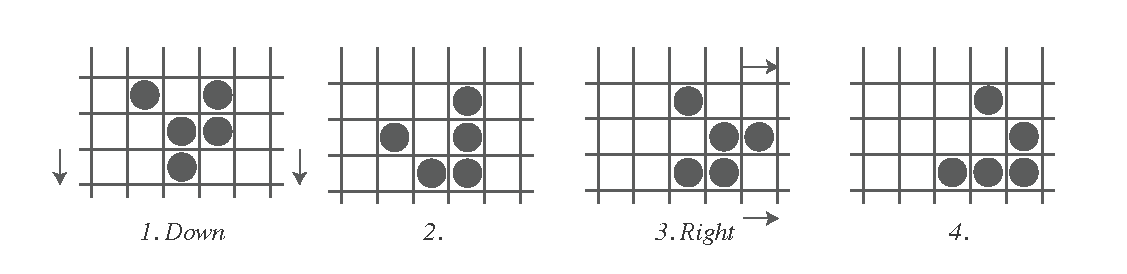
\includegraphics[width=0.9\textwidth, trim={0cm 0cm 0cm 0cm},clip]{Illustrations/Glider.pdf}
  \caption{The glider pattern in the "Game of Life" Cellular Automata is a periodic pattern. Each time it loops, it moves one step to the right and one step down (indicated by the little arrows.  )  }
      \label{fig:glider}
\end{figure}

When you study figure  \ref{fig:glider}, you must imagine this pattern going through frames 1 through 4, and then looping back to frame 1. The little arrows indicate frames where the pattern enters a new column or row that it has not previously touched. As you can see, every forth frame the glider only moves one steps to the right and one step down. This makes it propagate at an angle of $\theta  = -45 \degree$. However, if we rotate the pattern 90, 180 and 270 degrees the pattern can move in a total of four distinct directions. Let us coin the term Effective Directional Information (EDI), which is an integer and is the number of different directions that a pattern can move in. Because the glider can move in 4 directions, it's EDI number is 4. I It's not something that we can see directly, but somehwere in the intial configuration in the first frame of Figure \ref{fig:glider}, the future of the evolution is already determined, through a relation to the rules of Conways Game of Life. 

Several things are determined for this pattern, given the initial configuration. 

\begin{enumerate}
\item The direction of propagation ($-45\deg$).
\item The number of reorientations of the pattern possible (4)
\item The periodicity (also 4)
\item All intermediate steps

\end{enumerate}
The most compact way of storing this EDI number, would be as binary power-series. Therfore, we define the bitlength $b$, as the number of bits required to express the EDI number.

\begin{equation}
\label{eq:EDI}
EDI =  2^b
\end{equation}




Now it becomes intuitively clear, that the information pattern, our digital photon if you will, cannot contain infinite amount of data, because that means it would be infinitely large. Perhaps a better question is : How large does $b$ need to be, to create an EDI number where the photon can travel from anywhere in the observable universe to anywhere else in the observable universe, with absolute precision? Because that is what we are currently expecting photons to be able to do, through the equations we are using in physics. The answer depends again, on accuracy. In Quantum Mechanics however, there is a constant called Plancks Length $\ell_P$, which is currently defined to be $1.61622837 \times 10^{-35} m $ , and the size of the observable universe defined to be $8.8\times10^{26} m$ across. The observable universe therefore is $5.44 \times 10^{61}$ times larges that the Planck Length. 

\begin{equation}\label{eq:universesize}
2^b =  \frac{U_L}{\ell_P} = \frac{8.8\times10^{26} }{1.61622837 \times 10^{-35}} 
\end{equation}

Solving for b and rounding up gives us 204 bits. Not more, not less. This means that in order for a determinstic deep quantum photon to have virtually infinite directional freedom, as is ascribed to it by both  classical and quantum physics, it need no more than 204 bits of EDI to reach any point in the universe from any point, with perfect precision. This places an upper bound only. The lower bound, or the minimum amount of EDI that light needs to have to be able to appear is probably more interesting, and as it turns out - much more difficult and wrought with surprising twists.


\section{Lightlanes}
We can also work this the other way, going from a specified EDI to saying something about the pattern. Consider a photon with $2^b$ of EDI data about its precise direction through space. This limits the number of possible directions the light can travel to $2^b$ options from its origin. We refer to each of these possible escape paths as lightlanes represented by the vector $\vec{L}$, and the function $I(\vec{L})$ as the amount of information stored in a lightlane vector.

\begin{definition}{ Lightlane Information:}
Let $I(\vec{L})$ be a function returning the amount of information in a vector as an integer. $I(\vec{L})$ is equal to the number of dimensions plus the absolute value of each vector component, so that $I(\vec{L})  = |\vec{L}.x| +  |\vec{L}.y| + |\vec{L}.z| + 3$
\end{definition}
\begin{definition}{ Lightlane:}
A lightlane is a vector $\vec{L}$  through space from an origin. The amount of information stored in the lightlane vector cannot exceed the EDI of the pattern it belongs to. For a 3D vector,  $I (\vec{L}) <=  2^b$.
\end{definition}

\begin{figure}[!ht]
  \centering

 \includegraphics[width=0.8\textwidth, trim={0cm 0cm 0cm 0cm},clip]{Illustrations/lightlanes.pdf}
  \caption{Lightlanes with $b$ = 3 and 4. Lanes double for each increment of b. }
      \label{fig:1}
\end{figure}


\section{Photon Counter equation}

In order to proceed, we first set up a thought experiment. Let there be a point source of photons, emitting photons randomly in all directions. Place a detector occupying $D$ of the circumference at distance $d$ from the light source. The expected number of photons received $\tau_c $, equal the proportion of the detector to circumference at distance $d$. 

Let the classical expected photon count equation be:
\begin{equation}\label{eq:classicalPC}
\hat{\tau_c} =  \frac{D}{2 d\pi}E 
\end{equation}

If we emit 1000 photons from the centre, then this equation tells us the share of photons received by D. This can be simplfied by converting the length of D to the angle it occupies, $D_\theta$ in radians.

\begin{equation}\label{eq:classicalPCTheta}
\hat{\tau_c} =  \frac{D_\theta}{2 \pi}E 
\end{equation}

In Figure \ref{fig:thejuul}, right panel we can see that the detector $D$ intersects with exactly one lightlane. This gives us the opportunity to calulcate $\theta$,  the angle between lightlanes (\ref{eq:theta}), measured in radians. 

\begin{equation}
\theta = \frac{2\pi}{2^b}
\label{eq:theta}
\end{equation}



\begin{figure}[!ht]
  \centering

 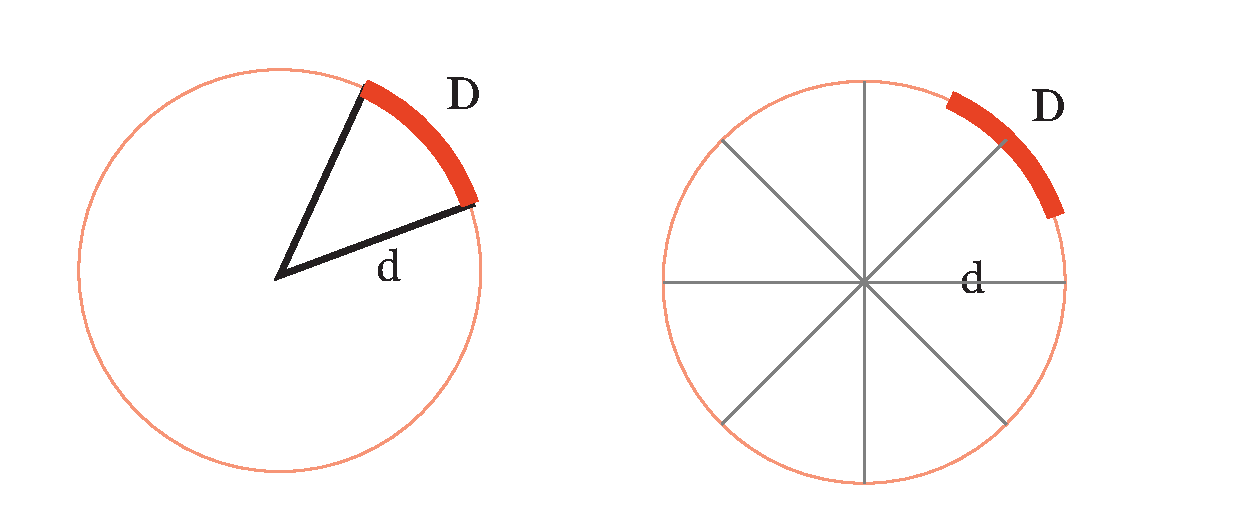
\includegraphics[width=0.8\textwidth, trim={0cm 0cm 0cm 0cm},clip]{Illustrations/Fig1_2.pdf}
  \caption{Left hand: $\tau_c$ : Detector $D$, distance $d$. Right hand: $\tau_x$ detector intersecting 1 lightlane, obtaining $\frac{1}{2^b}  = \frac{1}{8} =  $ of photons emitted, indicating a bitlength of 3, because  $ 8 = 2^b \rightarrow \sqrt[3]{8}  = 2  $ }
      \label{fig:thejuul}
\end{figure}

\begin{figure}[!ht]
  \centering

 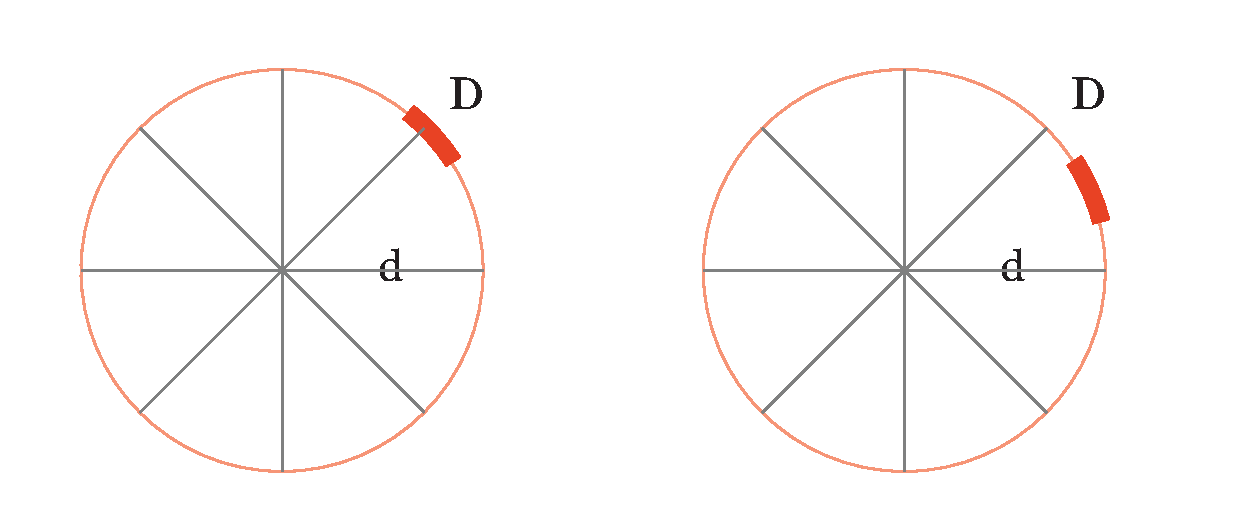
\includegraphics[width=0.8\textwidth, trim={0cm 0cm 0cm 0cm},clip]{Illustrations/Fig2.pdf}
  \caption{Left hand side : Detector is considerably smaller, but still, obtaining $\frac{1}{8} $ of photons emitted. Right hand side : Detector is in dark zone, receives no photons }
    \label{fig:SmallDetector}
\end{figure}

\section{The Lightlane Equality }

Recalling equation \ref{eq:classicalPCTheta}, let $D_\theta$ be the angle occupied by the detector. The expected number of lightlanes that a detector $D$ intersect with is given by the angle it occupies divided by the angle between lightlanes.

\begin{equation}
\hat{L} =   \frac{D_\theta }{ \theta} 
\label{eq:expectedLightlanes}
\end{equation}

The light emitted is now constrained to travel in $2^b$ lightlanes. This means that the expected number of photons per lightlane must be given by $\hat{E_L}$
\begin{equation}
 \hat{E_L} = \frac{E}{2^b}
 \label{eq:expectedPhotonsPerLane}
\end{equation}

We now have expected number of lightlanes $\hat{E}_L$ intersected by Detector $D$,  and expected photons per lane  $\hat{L}$. The expected total number of Photons on detector then becomes.
\begin{equation}\label{eq:TauXdefinitionShort}
\tau_x =  \hat{L} \hat{E_L} 
\end{equation}

Substituting $\hat{E_L}$ and $\hat{L} $ with equations, and simplifying give us.
\begin{equation}
 \tau_x = \frac{2^b D_\theta}{2\pi} \frac{E}{2^b} = \frac{2^b D_\theta E}{2^b2\pi} =  \frac{ D_\theta}{2 \pi} E 
 \label{eq:Lightlaneequality}
\end{equation}

Compare equations for $\hat{\tau_c} $ and $\hat{\tau_x} $ and notice how equation  \eqref{eq:Lightlaneequality} and  \eqref{eq:classicalPCTheta} are equal. This has a possible interpretation that is quite profound. If the expected value is exactly the same in both a infinite directional movement and in the Lightlane variant taking into account the amount of directional information the photon carries with it, the classical equation  $\hat{\tau_c} $ could well be an approximation for  $\hat{\tau_x} $, assuming high bitlength.


\section{Dark zones}
However, there is an important difference between  $ \tau_x $ \eqref{eq:TauXdefinitionShort} and $ \tau_c$ \eqref{eq:classicalPCTheta}  which comes into play as we vary the position of the emitter and detector.
While keeping in mind that  $\tau_x$  and $ \tau_c$ have the exact same Expected value( because the term $2^b$ disappears from the equation through simplification), this term isn't always irrelevant. In Figure \ref{fig:SmallDetector} we can see this in action : A tiny detector capturing an full $\frac{1}{8} $ of available photons, despite its minuscule share of the circumference at distance $d$. Clearly, the left hand in Figure \ref{fig:SmallDetector}  is overperforming and the right hand is underperforming given the expected value $\tau_c$. The difference between $\tau_c$ and $\tau_x$ is therefore affecting the variance. Intuitively we can see that as the number of lightlanes increases, the difference between $\sigma_x$ and $\sigma_c$ approaches zero.


As shown to the left panel in Figure \ref{fig:SmallDetector}, a carefully positioned detector, irrespective of it's size is able to receive $ \frac{1}{2^b}  $ of the photons emitted from this point, provided that the position remains fixed. In the special case where  $ D_\theta < \frac{2 \pi}{ 2^b} $ (Figure \ref{fig:SmallDetector}, right panel)  this clearly illustrates that the Observed Photon Count $T_x$ can be zero, which is very  different from the Expected Photon count $\hat{\tau_x}$. This is called a dark-zoned detector, charaterized by \ref{eq:darkZoneEquation}

\begin{equation}
 \tau_x = 0  \neq \hat{\tau_x}
 \label{eq:darkZoneEquation}
\end{equation}

This leads us to the first theorem:

\begin{theorem}
Lightlane Equality : The expected photon count $\tau_c$ for a classical point emitter equals that of directionally constrained emitter $\tau_x$ , if and only if their relative velocity is not zero.
\end{theorem}

\section{Lightlane Twinkle Density}
What if the detector is moving relative to the point emitter? In Figure \ref{fig:MovingDetector} the detector  moving at a steady pace around the circumference. In the right panel of Figure \ref{fig:MovingDetector}, the detector has moved 9 times its angle $D_\theta$, in the time $t$. It follows quite nicely that the decimal part of the expected lightlane  \eqref{eq:expectedLightlanes} correspond to intersecting an \textbf{additional} lane or not. 

\begin{figure}[!ht]
  \centering

 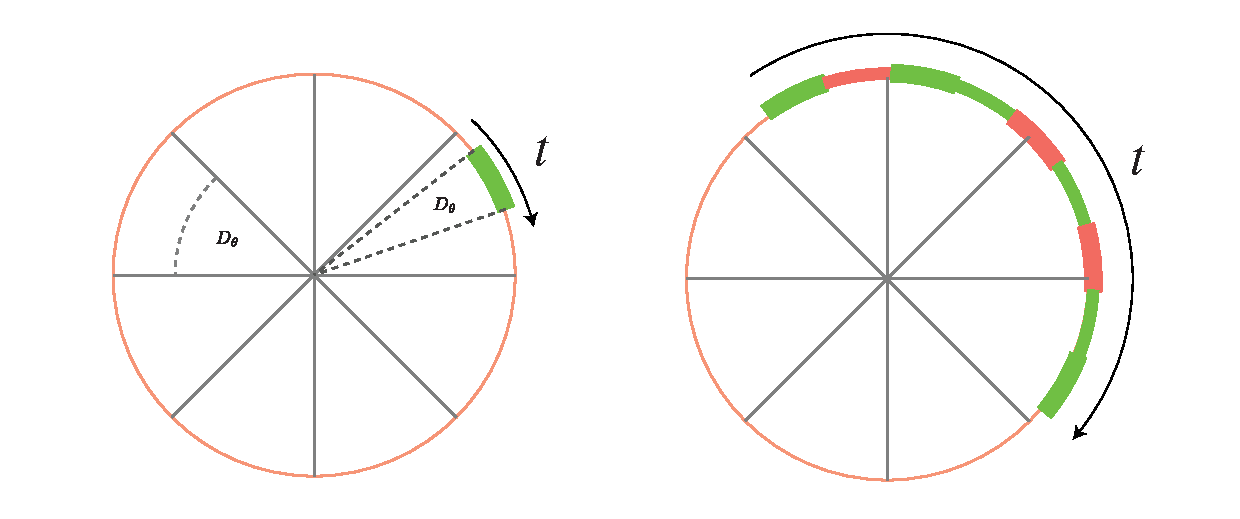
\includegraphics[width=0.8\textwidth, trim={0cm 0cm 0cm 0cm},clip]{Illustrations/Twinkle.pdf}
  \caption{Moving detector will either intersect with N lightlanes, or with N+1 lightlanes. }
    \label{fig:MovingDetector}
\end{figure}

Let us imagine expected lane count ($ \hat{L} $) is equal 2.54. This can then be interpreted as intersecting three lanes $54\%$ of the time, and two lanes $46\%$ of the time. We could, if we wanted to represent this as a probability distribution of the form: 


\begin{equation*}
C_{D_\theta, b} = f(D_\theta, b) = 
\begin{pmatrix}
n & p_n &  \\
n+1 & p_{n+1}\\
\end{pmatrix}
\end{equation*}

We name this special probability distribution \textbf{Twinkle}, because it makes the light twinkle. The Twinkle is an function of the detector angle $D_\theta,$ the bitlength $b$ and the distance $d$, returning an enumerated list of at least two adjacent positive integers with respective probabilities. The Twinkle is a proper density function, and hence the probabilities always sum to unity. The Twinkle for $\hat{L} = 2.54$ would be:

\begin{equation*}
\hat{L} = 2.53 =>  T
\begin{pmatrix}
2 & 0.46 &  \\
3 & 0.53 \\
\end{pmatrix}
\label{Twinkle254}
\end{equation*}

In the simple case where the detector angle $ D_\theta $ is the same during the entire photon collection, these probabilities do not change over time. This means photon collection can be explained from knowing a Twinkle, receiving three lightlanes and two in a ratio that produces the same expected photon count as the classical.

\begin{definition}{\large Twinkle:}
A Twinkle is a set of integers with associated probabilities, where the integers are always adjacent and the probabilities sum to unity.
\end{definition}

\begin{definition}{\large Simple Twinkle} 
A simple Twinkle is a Twinkle alternating between two lightlane numbers, and the Twinkle periodicity is short compared to capture time and the, probabilites do not change over time. I.e the direction $d$is fixed.
\end{definition}

It is also possible to reverse engineer Twinkles, working backwards from observed variance in flux. For example, if observed flux falls exactly 33.33\% from the peak periodically, we are likely to be observing a [2, 3] twinkle because 2 is 66\% of 3. The probabilities determine how much time we are observing 2 vs 3 lightlanes.

\section{Variance}
For any experimental setup where the detector is moving with a constant distance to the emitter, the mean value is also the expected photon count in \eqref{eq:classicalPCTheta} and \eqref{eq:Lightlaneequality}, so that  $\hat{\tau_x} = \hat{\tau_c}$. This equality only applies to the mean, not to the Variance. The variance  is  the expected value of \textbf{the square of the deviation from the mean}, and becomes a much more complex relationship due to the involvement of the bitlength $b$.

The conversion of the expected lane count $\hat{L}$ to a Twinkle object allows us to formalize a general definition for the Variance. Let the Twinkle under consideration be the Simple Twinkle in equation \eqref{Twinkle254}, toggling between a low (K=2) and a high (K=3) lanecount. 


\begin{equation}
	\sigma^2 = 0.54 \times (\frac{(2.54 - 3)E}{2^b})^2 + 0.46 \times (\frac{(2.54 - 2)E}{2^b})^2
	\label{eq:Twinkle254Variance}
\end{equation}

A generalized form of this using Twinkles, where $K_i$ is the lanecount, and $P_i$ the associated probability, is given as:

\begin{equation}
	\sigma^2 =  \left( \sum^T_{K_i, P_i \in T}  P_i (\frac{D_\theta E }{2\pi} - K_i \frac{E}{2^b})^2\right)N
	\label{eq:deviancefrommean}
\end{equation}

As you can see the second term of the variance becomes zero as the bitlength expression $2^b$ approaches infinity. For very high values of $b$, the variance equation simplify to:

\begin{equation}
	\sigma^2 =  \frac{D_\theta E }{2\pi} N
	\label{eq:deviancefrommeansimplified}
\end{equation}

DRAFT NOTE : The equation for VARIANCE is very likely incorrect, I appreciate help fixing it.

\section{Conclusion}
The Lightlane Equality is the first foray into exploring the consequences of the "Lightlane Argument", seeking a way to connect metaphysics with physics. This is possible due to a technicality arising from the axiomatic foundations of several information based, deterministic deep quantum theories. In these systems, the existence of an information "grid" and the identification of information with physical reality puts a constraint on the ability of light to take any direction through space without breaking the axiomatic foundations. Such deterministic, grid-based Deep Quantum theories can therefore be falsified by conclusively proving that light is not  constrained by carrying internal information. 
We have established in this paper, that when light has directional freedom (EDI) in the range where $b >= 204$,  the resolution is so high that it is completely indistinguishable from the classical, continous equations which assume infinite directional freedom. But if bitlength is much lower, it might have detectable effects. Due to the Lightlane equality however, such effects are likely to be subtle.
Another interesting find is that the expected value for the Lightlane photon counter simulation, is equal to the classical version, provided that the emitter and detector have a relative velocity. Another important find, is that while the mean is unaffected by bitlength in a moving frame, variance is not.
Because of this variance comes up as the most promising metric to study. To do this, we have introduced of a special class of probability densities called Twinkles. These formalize the exploration of bitlength sensitive variance.  On the low end, the minimal Twinkle is toggling between $K_i = 0$ and $K_i = 1$ yielding a very different Variance than the classical equation. This can be leveraged to constraining the bitlength, i.e the amount of Effective Directional Information (EDI) a photon can hold. Notably, the Twinkle can also be reverse engineered from observed Flux. If the bitlength is significantly lower than 204 bits, it might be possible to make predictions about photonic behaviour that is inconsistent with current formulations of classical physics as well as quantum physics that implicitly assume infinite directional freedom.


	


\bibliographystyle{plain}
\bibliography{mybib}






%\includegraphics[width=0.65\textwidth]{eps_demo}
\end{document}
